% =============================================================================
%  SECTION 2 — Background: RL → MARL → HARL
%  Slides 2.1–2.3  |  Target time: ~5 minutes
%
%  Purpose: establish shared vocabulary for the contributions.
%  The committee knows RL. Move efficiently — no tutorial.
% =============================================================================

%%==========================================================================
%% BACKGROUND
%%==========================================================================

\begin{frame}{Reinforcement Learning Essentials}
\begin{columns}
    \begin{column}{0.52\textwidth}
        \begin{block}{The MDP Tuple $({S},{A},P,r,\gamma)$}
            \begin{center}
                \renewcommand{\arraystretch}{1}
                \begin{tabular}{@{} l p{4.2cm} @{}}
                    $S$      & State space \\
                    $A$      & Action space \\
                    $P$      & Transition dynamics \\
                    $r$      & Reward function \\
                    $\gamma$ & Discount factor \\
                \end{tabular}
            \end{center}
        \end{block}
        \begin{itemize}
            \item \textbf{Policy} $\pi(a \mid s)$: probability distribution
                over actions given current state.
            \item \textbf{Objective}: find $\pi^{*}$ maximizing
                expected discounted return
                $\mathbb{E}_{\pi}\!\left[\sum_{t=0}^{\infty} \gamma^{t} r_t\right]$.
        \end{itemize}
    \end{column}
    \begin{column}{0.45\textwidth}
        \begin{figure}
            \centering
            \includegraphics[width=0.95\linewidth]{mdp_cycle.tex}
            \caption{The RL training loop: agent observes state, selects
                     action, receives reward, and updates policy.}
        \end{figure}
    \end{column}
\end{columns}

\note[item]{This isn't a tutorial on topicss}
\note[item]{
    This slide is provide clarity in \emph{notation}, 
    primarily drawn from Sutton and Barto / Albrecht and Christianos
}
\end{frame}


\begin{frame}[shrink=5]{Multi-Agent RL: The CTDE Paradigm}
\vspace{1.5em}
\begin{columns}
    \begin{column}{0.52\textwidth}

        \vspace{0.5em}
        \textbf{Centralized Training, Decentralized Execution (CTDE)}
        \cite{lowe2020,foerster2018}:
        \begin{itemize}
            \item \textbf{Training:} global state and joint actions
                available to the critic — reduces variance, improves
                credit assignment.
            \item \textbf{Execution:} each agent acts on
                \emph{local observations only} — deployable in the field.
        \end{itemize}
        \begin{itemize}
            \item \textbf{MAPPO}~\cite{yu2022}: CTDE actor-critic with
                optional parameter sharing across agents.
            \item All three contributions operate within this paradigm.
        \end{itemize}
    \end{column}
    \begin{column}{0.45\textwidth}
        \begin{figure}
            \centering
            \includegraphics[width=0.95\linewidth]{ctde_actor-critic.tex}
            \caption{CTDE actor-critic: global critic at training time;
                     local actors at execution time.}
        \end{figure}
    \end{column}
\end{columns}

\note[note]{Among most important MARL paradigms is CTDE}
\note[note]{Centralized control over training}
\note[note]{Deployabel to decentralized agents}
\note[note]{This is used for all three contributions}
\note[note]{Here I note MAPPO - typical of CTDE as actor-critic}
\note[note]{also used throughout}
\note[item]{\bfseries{Non-stationarity:} simultaneous updates may be individual
optimal, but suboptimal at the group level.
}
\end{frame}


\begin{frame}[shrink=10]{The Non-Stationarity Problem}
\vspace{2em}
\begin{columns}[c]
    \begin{column}{0.53\textwidth}
        \begin{block}{Definition}
            \(\pi\) optimization target changes over time,
            as a result of changes in environment, reward signals,
            or other agent's behaviors.
        \end{block}
        \begin{figure}
            \centering
            \includegraphics[width=\linewidth]{simultaneous_update.pdf}
            \caption{Effect of simultaneous v.\ sequential updates.}
        \end{figure}
    \end{column}
    \begin{column}{0.45\textwidth}
        \textbf{Three consequences:}
        \begin{enumerate}
            \item \textbf{Moving target.}
                Each agent optimizes against a policy
                that no longer exists by the next update.

            \item \textbf{Credit assignment.}
                A shared team reward $r$ gives no signal about
                \emph{which} agent's action helped or hurt.

            \item \textbf{Combinatorial explosion.}
                Joint action space grows as $k^n$ —
                intractable even for moderate team sizes.
        \end{enumerate}

    \end{column}
\end{columns}

\note[note]{Non-stationarity represents a moving target in your optimization}
\note[note]{Often results from dynamic environments}
\note[note]{In MARL we almost definitionally have a changing environment}
\note[note]{
    changing (other) agent behavior represents an environmental 
    change relative to the subject
}
\note[note]{
    \emph{The figure} shows the difference between simultaneous and
    sequential updates, which rep non-stationarity
}
\note[note]{
    \emph{If want example}: like trying to learn to play chess
    and every few moves you get a new opponent.
}
\note[note]{\textbf{Other consequences}}
\note[note]{Struggles with credit assignment}
\note[note]{
    Naive centralized control represents a combinatorial growth
    as a result of interactione
}
\end{frame}


\begin{frame}{Proximal Policy Optimization}
\begin{columns}[c]
    \begin{column}{0.44\textwidth}
        \begin{itemize}\small
            \item \textbf{$r_t > 1$:} policy moved \emph{toward} this action.
            \item \textbf{$r_t < 1$:} policy moved \emph{away} from it.
            \item Clipping kills the gradient outside
                $[1{-}\varepsilon,\,1{+}\varepsilon]$
                — large steps get no reward.
            \item In MARL: conservative updates dampen
                inter-agent non-stationarity~\cite{yu2022}.
        \end{itemize}
    \end{column}
    \begin{column}{0.54\textwidth}
        \begin{figure}
            \centering
            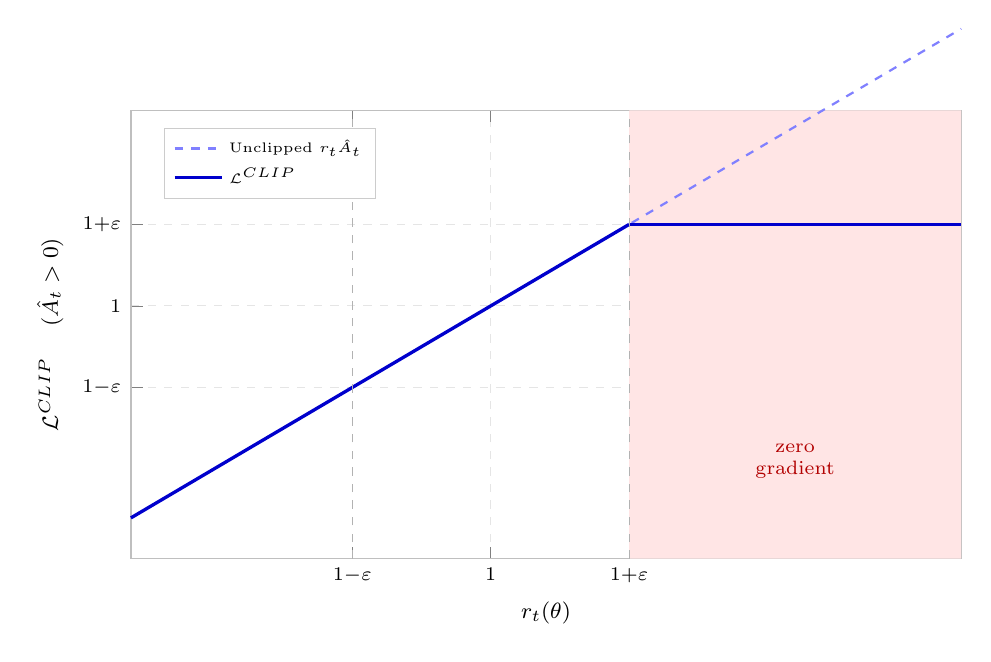
\begin{tikzpicture}
            \begin{axis}[
                width  = \linewidth,
                height = 0.6\linewidth,
                xmin=0.48, xmax=1.68,
                ymin=0.38, ymax=1.48,
                xlabel={$r_t(\theta)$},
                ylabel={$\mathcal{L}^{\text{CLIP}}$ \quad ($\hat{A}_t > 0$)},
                xlabel style={font=\footnotesize},
                ylabel style={font=\footnotesize},
                xtick={0.8, 1.0, 1.2},
                xticklabels={$1{-}\varepsilon$, $1$, $1{+}\varepsilon$},
                ytick={0.8, 1.0, 1.2},
                yticklabels={$1{-}\varepsilon$, $1$, $1{+}\varepsilon$},
                tick label style={font=\scriptsize},
                grid=major,
                grid style={dashed, gray!20},
                axis line style={gray!50},
                legend cell align=left,
                legend style={
                    font=\tiny,
                    at={(0.04,0.96)}, anchor=north west,
                    fill=white, draw=gray!40,
                },
                clip=false,
            ]
                %% Shaded dead zone: r > 1+eps, gradient = 0
                \addplot[fill=red!10, draw=none, forget plot]
                    coordinates {(1.2,0.38)(1.68,0.38)(1.68,1.48)(1.2,1.48)}
                    \closedcycle;

                %% Unclipped reference line
                \addplot[
                    blue!50, dashed, thick,
                    domain=0.48:1.68, samples=2,
                ] {x};
                \addlegendentry{Unclipped $r_t\hat{A}_t$}

                %% Clipped objective — linear up to 1+eps, then flat
                \addplot[
                    blue!80!black, very thick,
                    domain=0.48:1.2, samples=2,
                ] {x};
                \addplot[
                    blue!80!black, very thick,
                    domain=1.2:1.68, samples=2,
                ] {1.2};
                \addlegendentry{$\mathcal{L}^{\text{CLIP}}$}

                %% Vertical boundary lines
                \addplot[gray!60, thin, dashed]
                    coordinates {(0.8,0.38)(0.8,1.48)};
                \addplot[gray!60, thin, dashed]
                    coordinates {(1.2,0.38)(1.2,1.48)};

                %% Dead-zone annotation
                \node[
                    font=\scriptsize, text=red!70!black,
                    align=center,
                ] at (axis cs:1.44, 0.62) {zero\\gradient};
            \end{axis}
            \end{tikzpicture}
            \caption{\scriptsize Clipping prevents over-optimization:
                for a good action ($\hat{A}_t > 0$), once $r_t$ exceeds
                $1{+}\varepsilon$ the objective stops increasing.
                Mirror image holds for $\hat{A}_t < 0$.}
        \end{figure}
    \end{column}
\end{columns}
\begin{block}{}
    \centering\small
    $\mathcal{L}^{\text{CLIP}}(\theta)
        = \mathbb{E}_t\!\left[\,
            \min\!\left(
                r_t(\theta)\,\hat{A}_t,\quad
                \operatorname{clip}\!\left(r_t(\theta),\,
                    1{-}\varepsilon,\,1{+}\varepsilon\right)\hat{A}_t
            \right)
        \right]
    \qquad r_t(\theta) = \frac{\pi_\theta(a_t|s_t)}{\pi_{\theta_\text{old}}(a_t|s_t)}$
\end{block}

\note[note]{For most of my work I chose to stick with oen optimizer}
\note[item]{It is common}
\note[item]{It is stable}
\note[note]{\textbf{Clipping gives incidental benefits:}}
\note[item]{some resilience to non-stationarity}
\note[note]{smoothing on credit assignment}
\note[note]{more efficient than DDPG}
\end{frame}


% \begin{frame}{From MARL to HARL}

%     \small A natural progression: stronger heterogeneity handling
%     at increasing cost.

%     \vspace{0.6em}
%     \begin{center}
%     \renewcommand{\arraystretch}{1.5}
%     \begin{tabular}{@{} l c c c @{}}
%         \toprule
%         & \textbf{Parameter}
%         & \textbf{Heterogeneous}
%         & \textbf{Model} \\
%         & \textbf{Sharing}
%         & \textbf{Obs.\ Spaces}
%         & \textbf{Cost} \\
%         \midrule
%         \textbf{MAPPO}~\cite{yu2022}
%             & \textcolor{green!55!black}{\checkmark}
%             & \textcolor{red!60!black}{$\times$}
%             & $1\times$ \\
%         \textbf{HAPPO}~\cite{zhong2024}
%             & \textcolor{red!60!black}{$\times$}
%             & \textcolor{green!55!black}{\checkmark}
%             & $|\mathcal{I}|\times$ \\
%         % \hdashline\noalign{\vskip 4pt}
%         \textbf{This work}
%             & \textcolor{green!55!black}{\checkmark}
%             & \textcolor{green!55!black}{\checkmark}
%             & $1\times$ \\
%         \bottomrule
%     \end{tabular}
%     \end{center}

%     \vspace{0.4em}

%     \begin{columns}[t]
%         \begin{column}{0.52\textwidth}
%             \begin{block}{The Tradeoff Today}
%                 \small
%                 \textbf{MAPPO} shares parameters efficiently
%                     but requires $o_i \in \mathbb{R}^{d}$ for all $i$.\\[3pt]
%                 \textbf{HAPPO} handles $o_i \in \mathbb{R}^{d_i}$
%                     but trains a separate network per agent type —
%                     no cross-type learning, $|\mathcal{I}|\times$ storage.
%             \end{block}
%         \end{column}
%         \begin{column}{0.44\textwidth}
%             \begin{alertblock}{The Key Transition}
%                 Once agents differ \emph{structurally},
%                 the representation problem becomes
%                 \textbf{unavoidable} — and solving it
%                 recovers both sharing \emph{and} heterogeneity.
%             \end{alertblock}
%         \end{column}
%     \end{columns}

%     \note{About 2 minutes — this is the most important background slide.
%     Start at the top: ``Here is the landscape before this dissertation.''
%     Walk the table top to bottom.
%     MAPPO row: efficient, battle-tested, but the shared network
%     requires identical observation dimensions.
%     HAPPO row: handles heterogeneity rigorously — monotonic improvement
%     guarantees and all — but you pay with $|\mathcal{I}|$ separate
%     networks.  No parameter sharing means no cross-type transfer
%     and linear storage scaling.
%     Pause at the dashed line.
%     Say: ``The bottom row is what the next three contributions deliver.
%     The rest of this talk is the evidence.''
%     Then read the alertblock aloud as the transition.
%     HAPPO is our primary baseline in C2 and C3 precisely because
%     it represents the current best practice — our goal is to match
%     or beat it while collapsing the cost back to $1\times$.}
% \end{frame}

